\documentclass[%
pdf,
%nocolorBG,
colorBG,
slideColor,
%slideBW,
%draft,
%frames
%azure
%contemporain
%nuancegris
%troispoints
%lignesbleues
%darkblue
%alienglow
%autumn
]{prosper}
\usepackage{pifont, amsmath, multicol}
%\usepackage{floatflt, wrapfig,subfigure}
\usepackage{color}
\usepackage{epsfig}
\usepackage{pifont}
\usepackage[francais]{babel}
\usepackage[T1]{fontenc}
\usepackage[latin1]{inputenc}
\catcode`\�=\active
\catcode`\�=\active
\def�{\og\ignorespaces}%
\def�{{\fg}}%
\newcommand{\spacer}{\rule[-3mm]{0mm}{8mm}}
\newtheorem{theorem}{Theorem}
\newtheorem{definition}[theorem]{Definition}
\newtheorem{conjecture}[theorem]{Conjecture}
\newtheorem{corollary}[theorem]{Corollary}
\newtheorem{problem}[theorem]{Problem}
\newtheorem{lemma}{Lemma}
\newtheorem{claim}[theorem]{Claim}
\newtheorem{remark}[theorem]{Remark}
\newtheorem{proposition}[theorem]{Proposition}


\newcommand{\RR}{\ensuremath{\mathbb{R}}}
\newcommand{\NN}{\ensuremath{\mathbb{N}}}
\newcommand{\QQ}{\ensuremath{\mathbb{Q}}}
\newcommand{\CC}{\ensuremath{\mathbb{C}}}
\newcommand{\ZZ}{\ensuremath{\mathbb{Z}}}
\newcommand{\TT}{\ensuremath{\mathbb{T}}}

\def\QuotS#1#2{\leavevmode\kern-.0em\raise.2ex\hbox{$#1$}\kern-.1em/\kern-.1em\lower.25ex\hbox{$#2$}}


\title{\Huge \textcolor{blue}{Goldberg-Coxeter}\\[-1mm]
\textcolor{blue}{construction}\\[3mm]
\textcolor{blue}{for $3$- or $4$-valent}\\[4mm]
\textcolor{blue}{plane graphs}}
\author{\textcolor{red}{\large Mathieu Dutour}\\[2mm]
\textcolor{red}{\Large Hebrew University, Jerusalem}}
\slideCaption{}

\date{}



\begin{document}
\maketitle





\overlays{5}{
\begin{slide}{Goldberg-Coxeter for the Cube}
\onlySlide*{1}{\begin{center}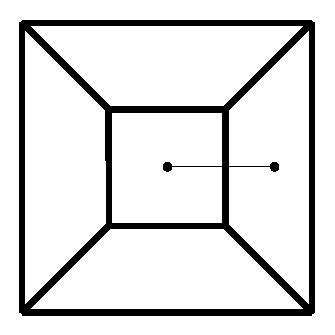
\epsfig{file=GOLDBERGpicture/Cube1_0-sec.eps,width=70mm}\end{center}}%
\onlySlide*{2}{\begin{center}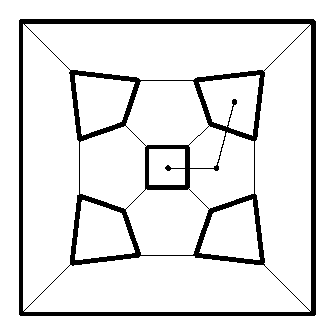
\epsfig{file=GOLDBERGpicture/Cube1_1-sec.eps,width=70mm}\end{center}}%
\onlySlide*{3}{\begin{center}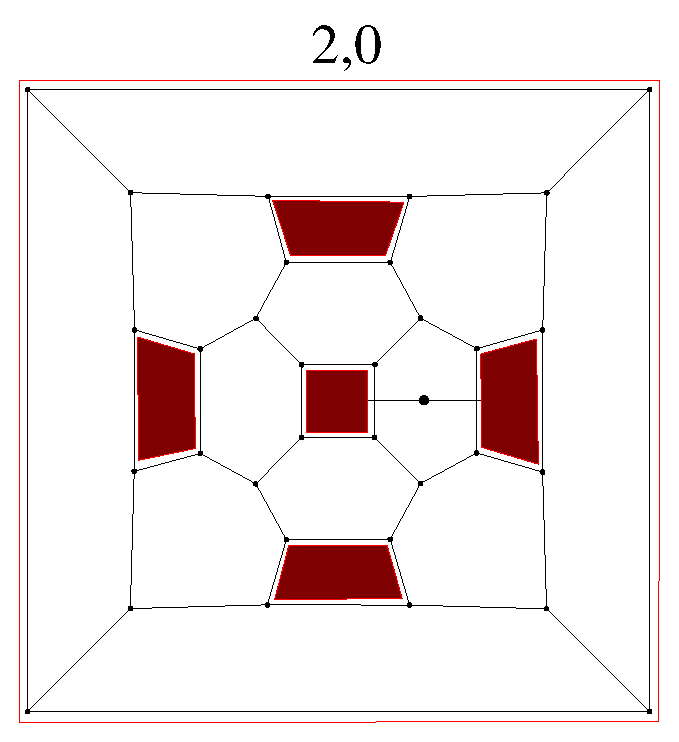
\epsfig{file=GOLDBERGpicture/Cube2_0-sec.eps,width=70mm}\end{center}}%
\onlySlide*{4}{\begin{center}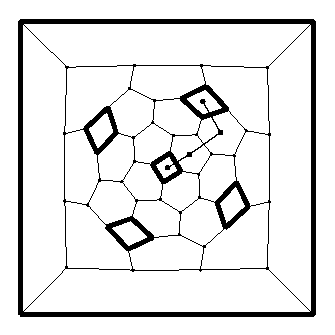
\epsfig{file=GOLDBERGpicture/Cube2_1-sec.eps,width=70mm}\end{center}}%
\onlySlide*{5}{\begin{center}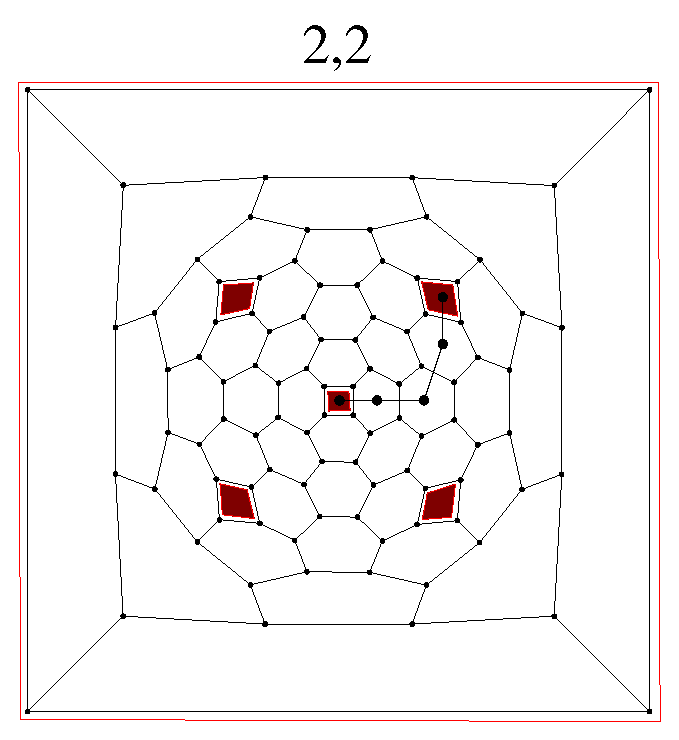
\epsfig{file=GOLDBERGpicture/Cube2_2-sec.eps,width=70mm}\end{center}}%

\end{slide}
}
















%%%%%%%%%%%%%%%   Slide synonyms
\overlays{4}{
\begin{slide}{History}

\onlySlide*{1}{{\bf Mathematics}: construction of planar graphs
\begin{center}
\begin{tabular}{p{10cm}}
M. Goldberg, {\em A class of multisymmetric polyhedra}, Tohoku Math. Journal, {\bf 43} (1937) 104--108.
\end{tabular}
\end{center}
\begin{equation*}
4_n=\left\{\begin{array}{c}
$3$-\mbox{valent~plane~graphs~with}\\
$4$\mbox{~or~}$6$\mbox{~gonal~faces}
\end{array}\right\}
\end{equation*}
{\em Goldberg theorem}: All graphs $4_n$ of symmetry $O$ or $O_h$ are obtained by his construction from the Cube.
}%
\onlySlide*{2}{{\bf Biology}: explanation of structure of icosahedral viruses
\begin{center}
\begin{tabular}{p{10cm}}
D.Caspar and A.Klug, {\em Physical Principles in the Construction of Regular Viruses},  Cold Spring Harbor Symp. Quant. Biol., {\bf 27} (1962) 1-24.
\end{tabular}
\end{center}
\begin{center}
\begin{tabular}{|c|c|c|}
\hline
$(k,l)$ & symmetry & capsid of virion\\
\hline
$(1,0)$ & $I_h$ & {\it gemini virus} \\
$(2,0)$ & $I_h$ & {\it hepathite B} \\
$(2,1)$ & $I$, laevo & {\it HK97, rabbit papilloma virus} \\
$(3,1)$ & $I$, laevo & {\it rotavirus} \\
$(4,0)$ & $I_h$ & {\it herpes virus, varicella} \\
$(5,0)$ & $I_h$ & {\it adenovirus} \\
$(6,3)$? & $I$, laevo & {\it HIV-1}\\
\hline
\end{tabular}
\end{center}
}%
\onlySlide*{3}{{\bf Architecture}: construction of geodesic domes

Patent by Buckminster Fuller
\begin{center}
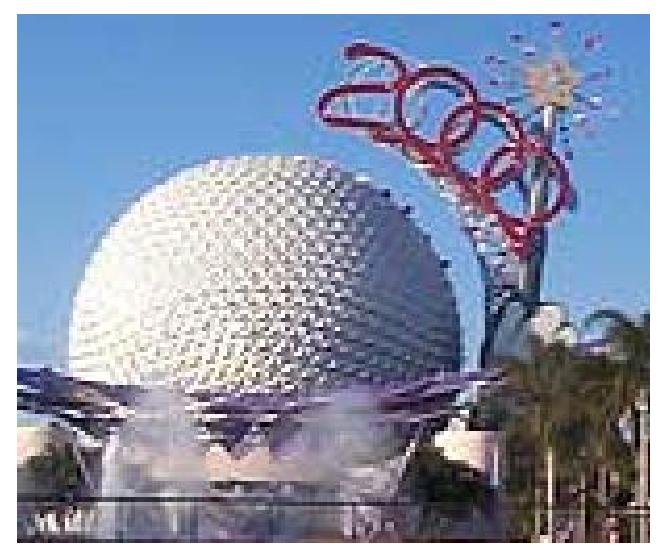
\epsfig{file=GOLDBERGpicture/2000spaceship-modified.eps,width=6.5cm}

EPCOT in Disney Land.
\end{center}
}%
\onlySlide*{4}{{\bf Mathematics}:
\begin{center}
\begin{tabular}{p{10cm}}
H.S.M. Coxeter, {\em Virus macromolecules and geodesic domes}, in {\em A spectrum of mathematics}; ed. by J.C.Butcher, Oxford University Press/Auckland University Press: Oxford, U.K./Auckland New-Zealand, (1971) 98--107.
\end{tabular}
\end{center}
}%



\end{slide}
}











%\maketitle
%\begin{slide}{PLAN}
%\renewcommand{\theenumi}{\textcolor{blue}{\Roman{enumi}}}
%\renewcommand{\labelenumi}{\theenumi.}
%\renewcommand{\theenumii}{\textcolor{blue}{\alph{enumii}}}
%\renewcommand{\labelenumii}{\theenumii.}
%
%\vspace{1.5cm}
%
%\begin{enumerate}
%\item \textcolor{red}{Zigzags and Central circuits}\\[0.5cm]
%
%\item \textcolor{red}{The Goldberg-Coxeter construction}\\[0.5cm]
%
%\item \textcolor{red}{The $(k,l)$-product}
%
%\end{enumerate}
%
%\end{slide}




%%%%%%%%%%%%%%%%%%%% Slide presentation
\begin{slide}{}
\begin{center}
{\Huge 
\begin{tabular*}{6cm}{c}
\\[-0.5cm]
\textcolor{blue}{I. }\textcolor{red}{ZigZags}\\
\textcolor{red}{and}\\
\textcolor{red}{central circuits}
\end{tabular*}
}
\end{center}
\end{slide}


%%%%%%%%%%%%%%   Central circuits
\overlays{6}{
\begin{slide}{Central circuits}
\onlySlide*{1}{\begin{center}\epsfig{file=GOLDBERGpicture/CentralCircuitSample1.eps,width=11cm}\end{center}}%
\onlySlide*{2}{\begin{center}\epsfig{file=GOLDBERGpicture/CentralCircuitSample2.eps,width=11cm}\end{center}}%
\onlySlide*{3}{\begin{center}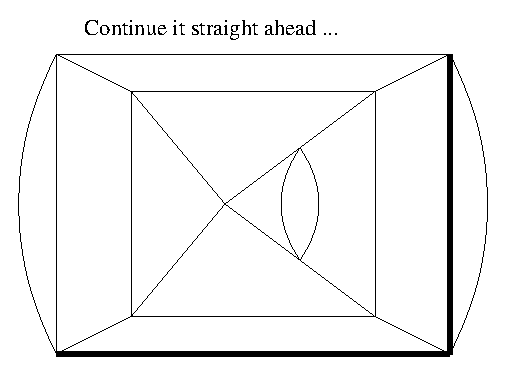
\epsfig{file=GOLDBERGpicture/CentralCircuitSample3.eps,width=11cm}\end{center}}%
\onlySlide*{4}{\begin{center}\epsfig{file=GOLDBERGpicture/CentralCircuitSample4.eps,width=11cm}\end{center}}%
\onlySlide*{5}{\begin{center}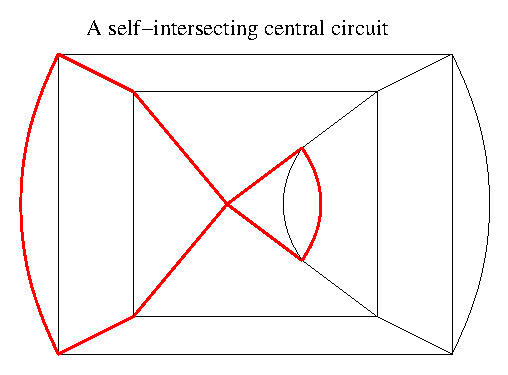
\epsfig{file=GOLDBERGpicture/CentralCircuitSample5.eps,width=11cm}\end{center}}%
\onlySlide*{6}{\begin{center}\epsfig{file=GOLDBERGpicture/CentralCircuitSample6.eps,width=9.8cm}\end{center}}%

\end{slide}
}


%ZIGZAGpicture/
\overlays{6}{
\begin{slide}{Zig Zags}
\onlySlide*{1}{\begin{center}\epsfig{file=ZIGZAGpicture/ZigZagSample1.eps,width=11cm}\end{center}}%
\onlySlide*{2}{\begin{center}\epsfig{file=ZIGZAGpicture/ZigZagSample2.eps,width=11cm}\end{center}}%
\onlySlide*{3}{\begin{center}\epsfig{file=ZIGZAGpicture/ZigZagSample3.eps,width=11cm}\end{center}}%
\onlySlide*{4}{\begin{center}\epsfig{file=ZIGZAGpicture/ZigZagSample4.eps,width=11cm}\end{center}}%
\onlySlide*{5}{\begin{center}\epsfig{file=ZIGZAGpicture/ZigZagSample5.eps,width=11cm}\end{center}}%
\onlySlide*{6}{\begin{center}\epsfig{file=ZIGZAGpicture/ZigZagSample6sharp.eps,width=9.8cm}\end{center}}%
\end{slide}
}





\begin{slide}{Notations}
\begin{enumerate}
\item[\ding{108}] \textcolor{red}{ZC-circuit} stands for ``zigzag or central circuit'' in $3$- or $4$-valent plane graphs.
\vspace{1cm}


\item[\ding{108}] The \textcolor{red}{length} of a ZC-circuit is the number of its edges.
\vspace{1cm}


\item[\ding{108}] The \textcolor{red}{ZC-vector} of a $3$- or $4$-valent plane graph $G_0$ is the vector $\dots, c_k^{m_k}, \dots$ where $m_k$ is the number of ZC-circuits of length $c_k$.
\vspace{1cm}

%\item[\ding{108}] A graph is ZC-transitive if its group of automorphism is transitive on the set of ZC-circuits

\end{enumerate}

\end{slide}



%%%%%%%%%%%%%  operators



%%%%%%%%%%%%%%%%%%%% Slide presentation
\begin{slide}{}
\begin{center}
{\Huge 
\begin{tabular*}{8cm}{c}
\\[-0.5cm]
\textcolor{blue}{II. }\textcolor{red}{Goldberg-Coxeter}\\
\textcolor{red}{construction}
\end{tabular*}
}
\end{center}
\end{slide}

%%%%%%%%%%%%%%%%%%%%  the construction
\begin{slide}{The construction}
\begin{enumerate}
\item[\ding{108}] Take a $3$- or $4$-valent plane graph $G_0$. The graph $G_0^{*}$ is formed of triangles or squares.
\item[\ding{108}] Break the triangles or squares into pieces:
\end{enumerate}
\begin{center}
\epsfig{file=GOLDBERGpicture/GoldbergBreakdown.eps,width=115mm}
\end{center}

\end{slide}


%%%%%%%%%%%%%%%%%%% sequel of construction
\begin{slide}{}
\begin{enumerate}
\item[\ding{108}] Glue the pieces together in a coherent way.
\item[\ding{108}] We obtain another triangulation or quadrangulation of the plane. 
\item[\ding{108}] Go to the dual and obtain the Goldberg-Coxeter construction, which is denoted $GC_{k,l}(G_0)$.
\end{enumerate}

%\vspace{1cm}
%This constructions extends to $3$- or $4$-valent oriented maps 
\end{slide}



%%%%%%%%%%%% an example at length.

\overlays{4}{
\begin{slide}{Example of $GC_{3,2}(Octahedron)$}
\onlySlide*{1}{\begin{center}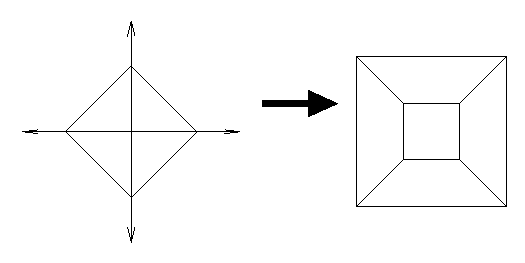
\epsfig{file=GOLDBERGpicture/Octahedron.eps,width=80mm}\end{center}}%
\onlySlide*{2}{\begin{center}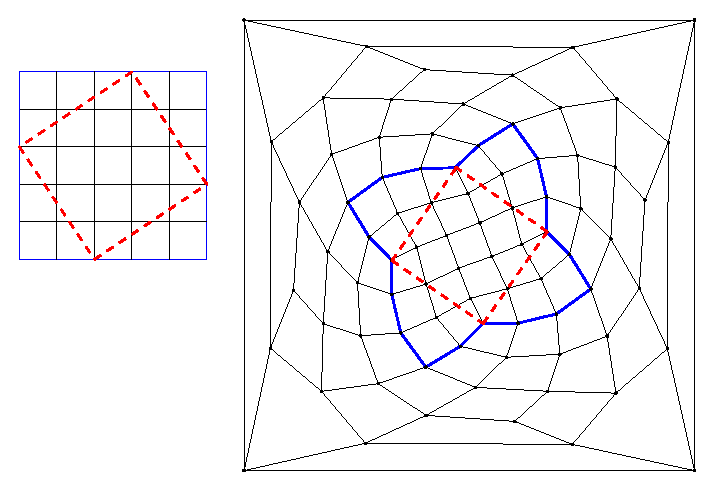
\epsfig{file=GOLDBERGpicture/dualPL32sec.eps,width=80mm}\end{center}}%
\onlySlide*{3}{\begin{center}\epsfig{file=GOLDBERGpicture/dualPL32secSquares.eps,width=80mm}\end{center}}%
\onlySlide*{4}{\begin{center}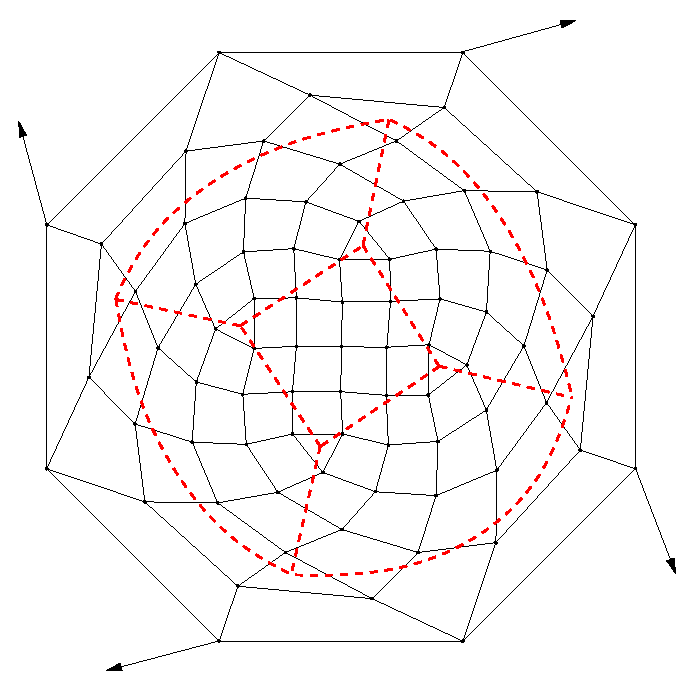
\epsfig{file=GOLDBERGpicture/nPL32thi.eps,width=80mm}\end{center}}%
\end{slide}
}






\begin{slide}{Properties}
\begin{enumerate}
\item[\ding{108}] One associates \textcolor{red}{$z=k+le^{i\frac{\pi}{3}}$(Eisenstein integer)} or \textcolor{red}{$z=k+li$(Gaussian integer)} to the pair $(k,l)$ in $3$- or $4$-valent case.

\item[\ding{108}] If one writes \textcolor{red}{$GC_{z}(G_0)$} instead of $GC_{k,l}(G_0)$, then one has:
\begin{equation*}
\begin{array}{rcl}
GC_{z}(GC_{z'}(G_0))  &=&GC_{zz'}(G_0)
%GC_{\overline{z}}(G_0)&=&GC_{z}(\overline{G_0})
\end{array}
\end{equation*}
%with $\overline{G_0}$ the symmetric on a plane of $G_0$.

%\item[\ding{108}] $GC_{1,0}(G_0)=G_0$
\item[\ding{108}] If $G_0$ has $n$ vertices, then $GC_{k,l}(G_0)$ has 
\begin{center}
\begin{tabular}{rcl}
$n(k^2+kl+l^2)=n|z|^2$ vertices &if& $G_0$ is $3$-valent,\\
$n(k^2+l^2)=n|z|^2$ vertices &if& $G_0$ is $4$-valent.
\end{tabular}
\end{center}

\end{enumerate}

\end{slide}



%%%%%%%%%%%%% medial and leapfrog
%\overlays{3}{
%\begin{slide}{The case $(k,l)=(1,1)$}
%\fromSlide{1}{
%\ding{108} For any $3$-valent plane graph $G_0$ the graph $GC_{1,1}(G_0)$ is called leapfrog of $G_0$.
%}
%\onlySlide*{1}{
%\begin{center}
%\begin{minipage}{5.5cm}
%\centering
%\epsfig{file=ExampleLeapFrog1.eps,width=50mm}\par
%Case $3$-valent
%\end{minipage}
%\begin{minipage}{5.5cm}
%\centering
%\epsfig{file=ExampleMedial1.eps,width=50mm}\par
%\vspace{0.9cm}
%Case $4$-valent
%\end{minipage}
%\end{center}
%}%
%\onlySlide*{2}{
%\begin{center}
%\begin{minipage}{5.5cm}
%\centering
%\epsfig{file=ExampleLeapFrog2.eps,width=50mm}\par
%Case $3$-valent
%\end{minipage}
%\begin{minipage}{5.5cm}
%\centering
%\epsfig{file=ExampleMedial2.eps,width=50mm}\par
%\vspace{0.9cm}
%Case $4$-valent
%\end{minipage}
%\end{center}
%}%
%\onlySlide*{3}{
%\begin{center}
%\begin{minipage}{5.5cm}
%\centering
%\epsfig{file=ExampleLeapFrog3.eps,width=50mm}\par
%Case $3$-valent\par
%$GC_{1,1}$ is called leapfrog
%\end{minipage}
%\begin{minipage}{5.5cm}
%\centering
%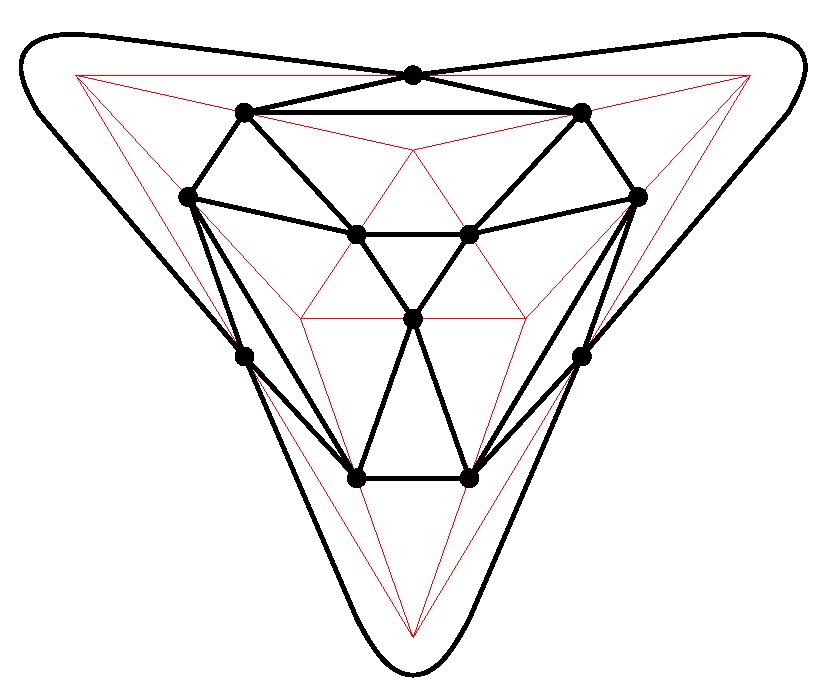
\epsfig{file=ExampleMedial3.eps,width=50mm}\par
%\vspace{0.9cm}
%Case $4$-valent\par
%$GC_{1,1}$ is called medial
%\end{minipage}
%\end{center}
%}%
%\ding{108} For any $4$-valent plane graph $G_0$ the graph $GC_{1,1}(G_0)$ is called medial graph of $G_0$.
%\end{slide}
%}


%%%%%%%%%%%%%%   Goldberg Theorem's
\begin{slide}{Goldberg Theorem}
\begin{enumerate}
\item[\ding{108}] \textcolor{red}{$q_n$} is the class of $3$-valent plane graphs having only $6$-gonal and $q$-gonal faces.
\item[\ding{108}] The class of $4$-valent plane graphs having only $4$- or $3$-gonal faces is called \textcolor{red}{Octahedrites}.
\end{enumerate}



\begin{center}
{\small
\begin{tabular}{|c|c|c|c|}
\hline
Class&             &Groups    &Construction\\
\hline
$3_n$&$p_3=4$      &$T$, $T_d$&$GC_{k,l}(\mbox{Tetrahedron})$\\
$4_n$&$p_4=6$      &$O$, $O_h$&$GC_{k,l}(\mbox{Cube})$\\
$5_n$&$p_5=12$     &$I$, $I_h$&$GC_{k,l}(\mbox{Dodecahedron})$\\
Octahedrites&$p_4=8$&$O$, $O_h$&$GC_{k,l}(\mbox{Octahedron})$\\
\hline
\end{tabular}
}
\end{center}




\end{slide}






%%%%%%%%%%%%%%  k-inflation theorem
\overlays{3}{
\begin{slide}{Zigzags and central circuits}
\fromSlide{1}{
\begin{enumerate}
\item[\ding{108}] Any ZC-circuit of $G_0$ corresponds to $k$ ZC-circuits of $GC_{k,0}(G_0)$ with length multiplied by $k$.
\item[\ding{108}] If the ZC-vector of $G_0$ is $\dots, c_l^{m_l}, \dots$, then the ZC-vector of $GC_{k,0}(G_0)$ is $\dots, (kc_l)^{km_l}, \dots$.
\end{enumerate}
}
\onlySlide*{1}{
\begin{center}
\begin{minipage}{5.5cm}
\centering
\epsfig{file=GOLDBERGpicture/Cube10Sec.eps,width=50mm}
\end{minipage}
\begin{minipage}{5.5cm}
\centering
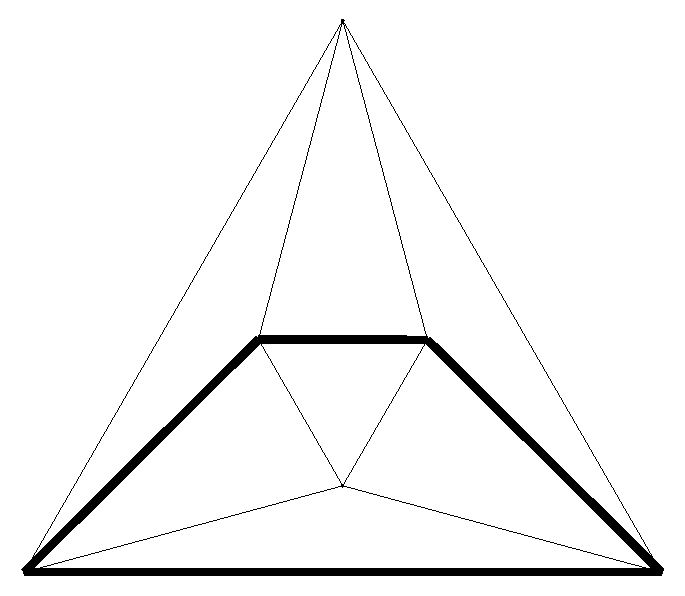
\epsfig{file=GOLDBERGpicture/Octahedron10Sec.eps,width=50mm}
\end{minipage}
\end{center}
}%
\onlySlide*{2}{
\begin{center}
\begin{minipage}{5.5cm}
\centering
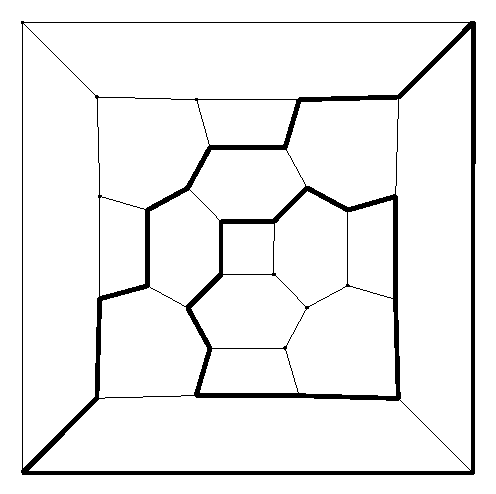
\epsfig{file=GOLDBERGpicture/Cube20Sec.eps,width=50mm}
\end{minipage}
\begin{minipage}{5.5cm}
\centering
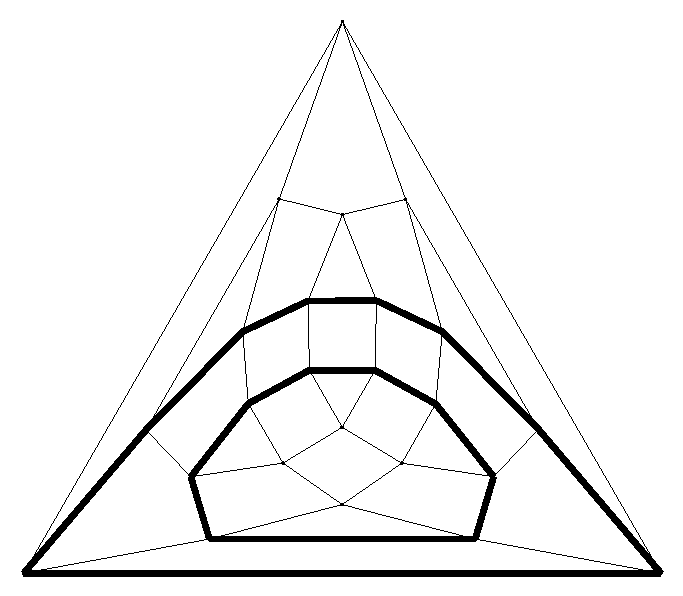
\epsfig{file=GOLDBERGpicture/Octahedron20Sec.eps,width=50mm}
\end{minipage}
\end{center}
}%
\onlySlide*{3}{
\begin{center}
\begin{minipage}{5.5cm}
\centering
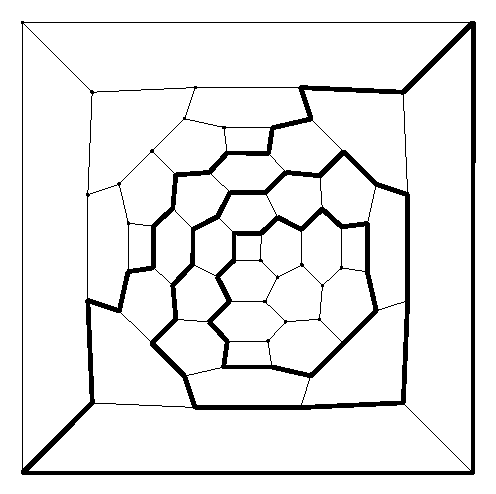
\epsfig{file=GOLDBERGpicture/Cube30Sec.eps,width=50mm}
\end{minipage}
\begin{minipage}{5.5cm}
\centering
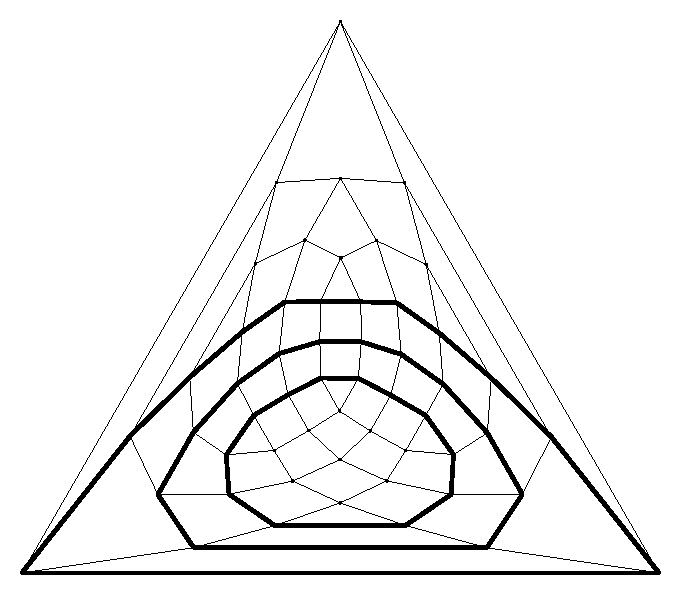
\epsfig{file=GOLDBERGpicture/Octahedron30Sec.eps,width=50mm}
\end{minipage}
\end{center}
}%

\end{slide}
}




%%%%%%%%%%%%%%%%%%%% The (k,l)-product
\begin{slide}{}
\begin{center}
{\Huge 
\begin{tabular*}{6cm}{c}
\\[-0.5cm]
\textcolor{blue}{III. }\textcolor{red}{The}\\
\textcolor{red}{$(k,l)$-product}
\end{tabular*}
}
\end{center}
\end{slide}





%%%%%%%%%%%%%%%%%%%%   the mapping phi_{k,l}

\begin{slide}{The mapping $\phi_{k,l}$}
\textcolor{red}{We always assume $gcd(k,l)=1$}

\begin{equation*}
\left\lbrace\begin{array}{rcl}
\textcolor{red}{\phi_{k,l}}:\{1,\dots, k+l\}  &\rightarrow   &\{1,\dots, k+l\}\\
u                             &\mapsto       &\left\lbrace\begin{array}{rcl}
u+l  &\mbox{~if~}   &u\in \{1,\dots, k\}\\
u-k  &\mbox{~if~}   &u\in \{k+1,\dots, k+l\}\\
\end{array}\right.
\end{array}\right.
\end{equation*}
is bijective and periodic with period $k+l$.

Case $k=5$, $l=2$:
\begin{equation*}
\begin{array}{l}
\phi^{(s)}(1)=1, 3, 5, 7, 2, 4, 6, 1, \dots\\
\mbox{operations:} (+2), (+2), (+2), (-5), (+2), (+2), (-5)
\end{array}
\end{equation*}


\end{slide}


\begin{slide}{The $(k,l)$-product}

\begin{enumerate}
\item[\ding{108}]
\begin{definition}(The $(k,l)$-product) 

If $L$ and $R$ are two elements of a group and $k,l\geq 0$ and $gcd(k,l)=1$; we define\\
$(p_0, \dots, p_{k+l})$ by $p_0=1$ and $p_{i}=\phi_{k,l}(p_{i-1})$.

Set \textcolor{red}{$S_i=L$} if $p_{i}-p_{i-1}=l$ and \textcolor{red}{$S_i=R$} if $p_{i}-p_{i-1}=-k$; then set
\begin{equation*}
\textcolor{red}{L\odot_{k,l} R=S_{k+l}\dots S_{2}\cdot S_{1}}.
\end{equation*}
By convention, set $L \odot_{1,0} R=L$ and $L\odot_{0,1} R=R$.\\
\end{definition}
For $k=5$, $l=2$, one gets the expression
\begin{equation*}
L\odot_{5,2} R=RLLRLLL
\end{equation*}


\end{enumerate}
\end{slide}


%%%%%%%%%%%   sequel of (k,l)-product
\begin{slide}{Properties}
\begin{enumerate}
\item[\ding{108}] If $L$ and $R$ commute, $L \odot_{k,l} R=L^k R^l$
\item[\ding{108}] Euclidean algorithm formula
\begin{equation*}
\left\lbrace\begin{array}{rcrcll}
L\odot_{k,l} R&=&  L   &\odot_{k-ql,\mbox{~~}l}&RL^q  &\mbox{if~}k-ql\geq 0\\
L\odot_{k,l} R&=&  R^qL&\odot_{k\mbox{~~}, l-qk}&R     &\mbox{if~}l-qk\geq 0
\end{array}\right.
\end{equation*}

\item[\ding{224}] If $L$ and $R$ do not commute, then $L\odot_{k,l} R\not= Id$.

\end{enumerate}
\end{slide}


%%%%%%%%%%%%%%%%%%%% The (k,l)-product
\begin{slide}{}
\begin{center}
{\Huge 
\begin{tabular*}{6cm}{c}
\\[-0.5cm]
\textcolor{blue}{IV. }\textcolor{red}{ZC-circuits}\\
\textcolor{red}{in}\\
\textcolor{red}{$GC_{k,l}(G_0)$}
\end{tabular*}
}
\end{center}
\end{slide}





%%%%%%%%%%%%%%%%%  the position mapping 
\overlays{6}{\begin{slide}{Position mapping, $3$-valent case}
\onlySlide*{1}{\begin{center}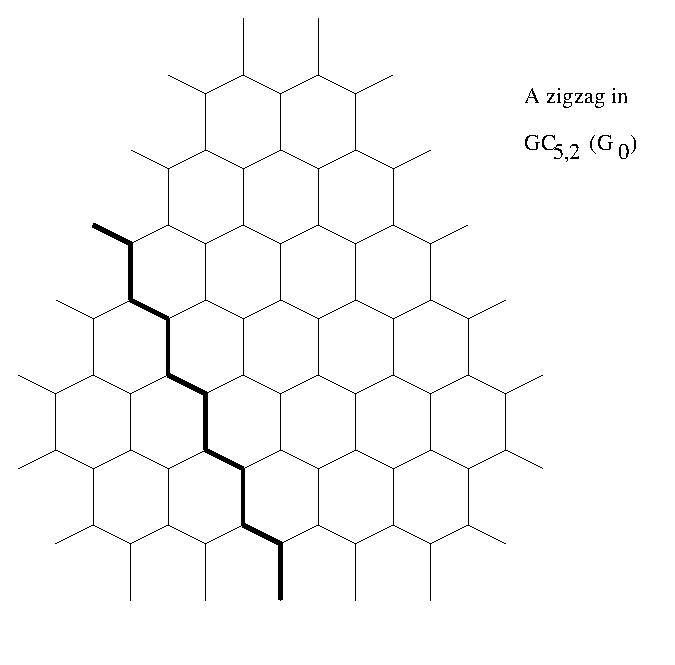
\epsfig{file=GOLDBERGpicture/PositionMapping3-Valent0-1.eps,width=80mm}\end{center}}%
\onlySlide*{2}{\begin{center}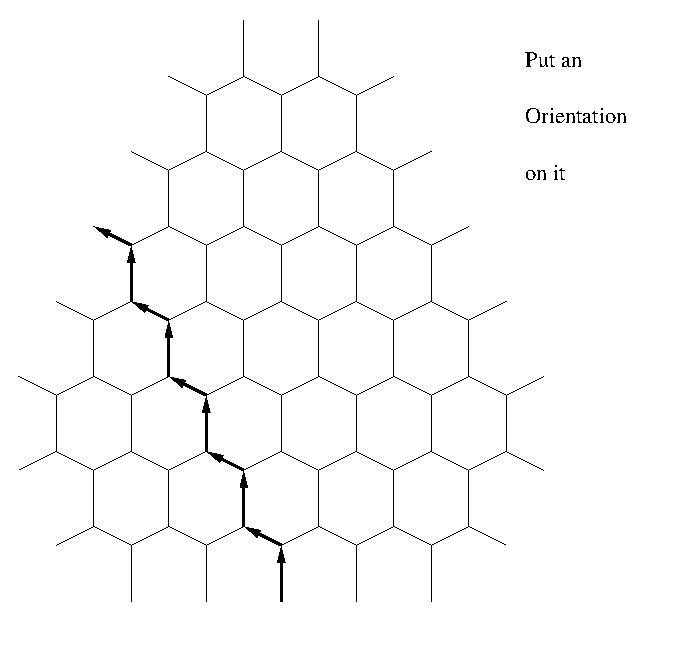
\epsfig{file=GOLDBERGpicture/PositionMapping3-Valent0-2.eps,width=80mm}\end{center}}%
\onlySlide*{3}{\begin{center}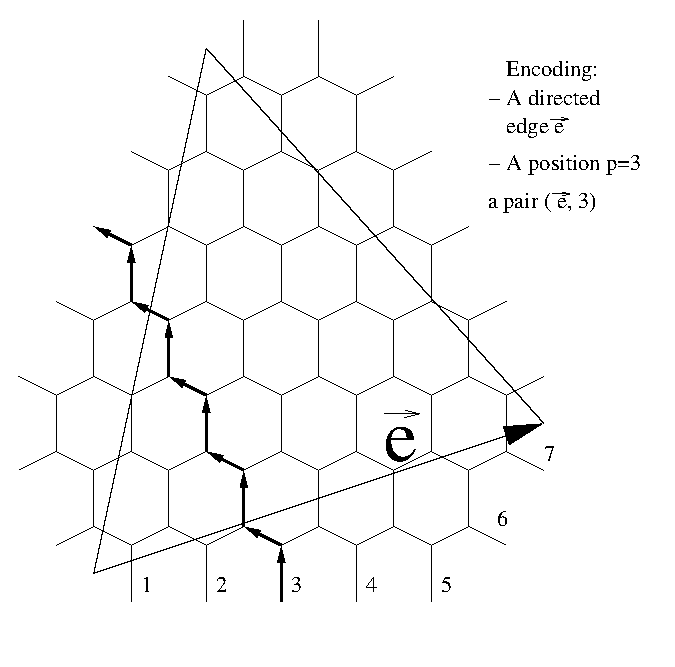
\epsfig{file=GOLDBERGpicture/PositionMapping3-Valent1.eps,width=80mm}\end{center}}%
\onlySlide*{4}{\begin{center}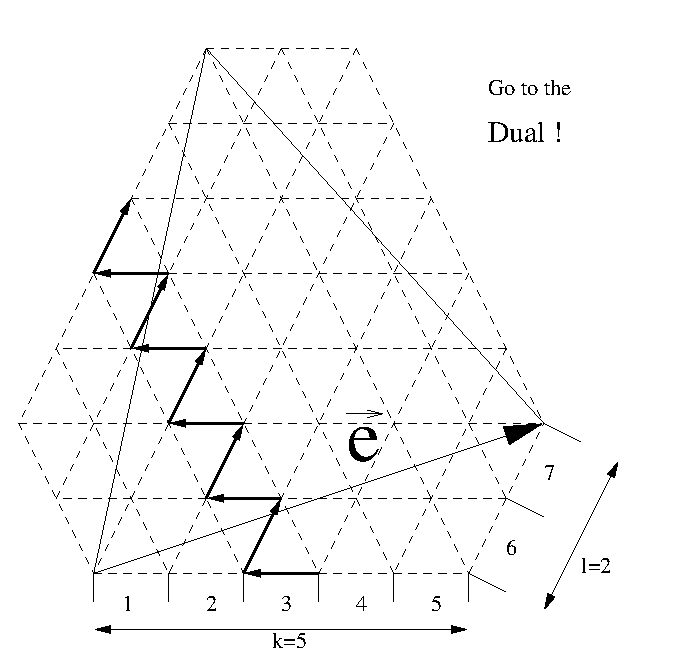
\epsfig{file=GOLDBERGpicture/PositionMapping3-Valent2.eps,width=80mm}\end{center}}%
\onlySlide*{5}{\begin{center}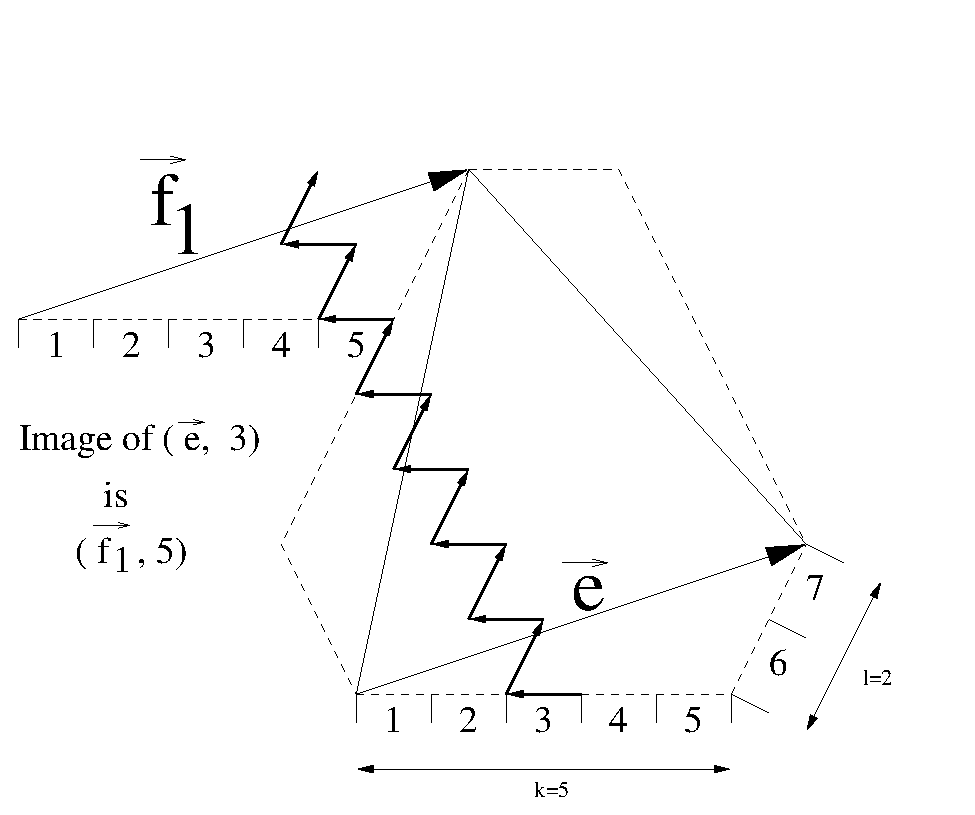
\epsfig{file=GOLDBERGpicture/PositionMapping3-Valent3.eps,width=90mm}\end{center}}%
\onlySlide*{6}{\begin{center}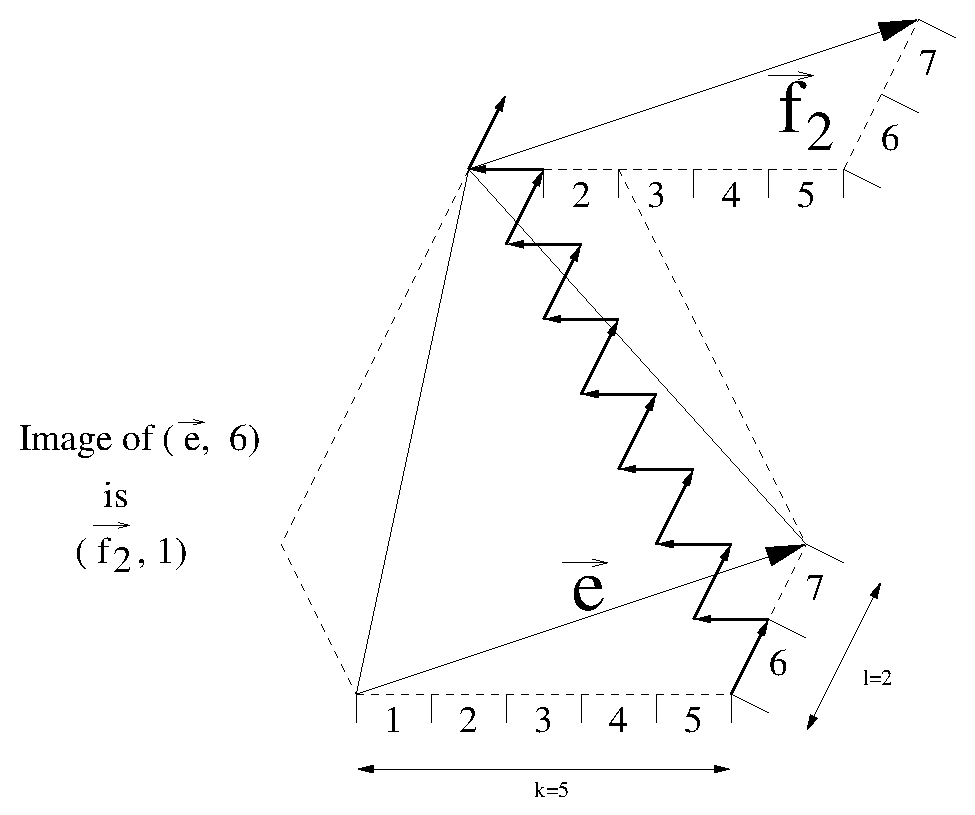
\epsfig{file=GOLDBERGpicture/PositionMapping3-Valent4.eps,width=90mm}\end{center}}%

\end{slide}
}


%%%%%%%%%%%%%%%%  Iterating the position mapping


\begin{slide}{Iteration}
\begin{enumerate}
\item[\ding{108}] We define \textcolor{red}{$PM(\overrightarrow{e}, p)$}=\textcolor{red}{$(\overrightarrow{f}_1, \phi_{k,l}(p))$} or \textcolor{red}{$(\overrightarrow{f}_2, \phi_{k,l}(p))$}
\item[\ding{108}] $PM^{k+l}(\overrightarrow{e}, 1)$=$(\overrightarrow{e'}, 1)$. So, one define \textcolor{red}{$IPM(\overrightarrow{e})=\overrightarrow{e'}$}.
\item[\ding{108}] For every ZC-circuit with pair $(\overrightarrow{e}, 1)$ denote \textcolor{red}{$Ord(ZC)$} the smallest $s>0$ such that $IPM^s(\overrightarrow{e})=\overrightarrow{e}$.
\item[\ding{224}] For any ZC-circuit of $GC_{k,l}(G_0)$ one has
\begin{tabular}{lll}
${\rm length}(ZC)$=$2(k^2+kl+l^2)Ord(ZC)$& $3$-valent case\\
${\rm length}(ZC)$=$(k^2+l^2)Ord(ZC)$ & $4$-valent case
\end{tabular}

If ZC of $GC_{k,l}(G_0)$ is \dots, $c_k^{m_k}$,\dots then \textcolor{red}{[ZC]} of $GC_{k,l}(G_0)$ is \dots, $\{\frac{c_k}{2(k^2+kl+l^2)}\}^{m_k}$,\dots or \dots, $\{\frac{c_k}{k^2+l^2}\}^{m_k}$,\dots.


%\item[\ding{108}] Denote [ZC]=
% the ZC-vector of $GC_{k,l}(G_0)$ with $c_k$ being the length divided by $2(k^2+kl+l^2)$ or $k^2+l^2$.
\end{enumerate}
\end{slide}



%%%%%%%%%%%%%%%%%%%%  computation of IPM

\begin{slide}{The mappings $L$ and $R$}
\begin{enumerate}
\item[\ding{108}] \textcolor{red}{${\cal DE}$} is the set of directed edges of $G_0^*$
\item[\ding{108}] \textcolor{red}{$L$} and \textcolor{red}{$R$} are the following permutation of ${\cal DE}$
\begin{equation*}
\textcolor{red}{L:\overrightarrow{e}\rightarrow\overrightarrow{f}_1}
\mbox{~~~~~~~~~~~~~}
\textcolor{red}{R:\overrightarrow{e}\rightarrow\overrightarrow{f}_2}
\end{equation*}
with $\overrightarrow{f}_1$ and $\overrightarrow{f}_2$ being the first and second choice.
\item[\ding{108}] \textcolor{red}{$Mov(G_0)=\langle L, R\rangle$} is the \textcolor{red}{moving group}
\item[\ding{108}] For $u\in Mov(G_0)$, denote \textcolor{red}{$ZC(u)$} the vector $\dots, c_k^{m_k},\dots$ with multiplicities $m_k$ being the \textcolor{red}{half of the number of cycles of length $c_k$} in the permutation $u$ acting on the set ${\cal DE}$.
\item[\ding{224}] One has
\textcolor{blue}{$[ZC]\mbox{~of~}GC_{k,l}(G_0)= ZC(L\odot_{k,l} R)$}



\end{enumerate}
\end{slide}





%%%%%%%%%%%   sequel of (k,l)-product
%\begin{slide}{Fundamental Theorem}
%\begin{enumerate}
%\end{enumerate}
%\end{slide}







%%%%%% the case of cube
\begin{slide}{The case of Cube}
\begin{enumerate}
\item[\ding{108}] $L$ and $R$ do not commute \ding{224} $L\odot_{k,l} R\not= Id$.
\item[\ding{108}] $Mov(Cube)=\langle L, R\rangle$=\textcolor{red}{$Alt(4)$}
\item[\ding{108}] $K=\langle (1,2)(3,4),(1,3)(2,4)\rangle$ \textcolor{red}{normal subgroup of index $3$} of $Alt(4)$. $\overline{L}$ is of \textcolor{red}{order $3$.}
\begin{equation*}
\left\lbrace\begin{array}{c}
\overline{L\odot_{k,l}R}=\overline{L}^k\overline{R}^l=\overline{L}^{k-l}\\
L\odot_{k,l}R\in K\Leftrightarrow k-l\mbox{~divisible~by~}3
\end{array}\right.
\end{equation*}
\item[\ding{108}] Elements of $Alt(4)-K$ have \textcolor{red}{order $3$}. Elements of $K-\{Id\}$ have \textcolor{red}{order $2$}.
\item[\ding{224}] $GC_{k,l}(\mbox{Cube})$ has \textcolor{blue}{[ZC]=$2^6$} if $k\equiv l\pmod 3$ and \textcolor{blue}{[ZC]=$3^4$}, otherwise
\end{enumerate}


\end{slide}





%%%%%%%%%%%%%%%%   the problems
%\begin{slide}{The two problems}
%
%\begin{enumerate}
%\item[\ding{224}] Compute the set of all possible [ZC] for $GC_{k,l}(G_0)$
%\begin{center}
%\begin{tabular}{p{8cm}}
%Solvable in finite time for a given $G_0$
%\end{tabular}
%\end{center}
%\vspace{1cm}
%
%\item[\ding{224}] Compute [ZC] in terms of the pair $(k,l)$
%\begin{center}
%\begin{tabular}{p{8cm}}
%Solvable in some cases.\\
%There is a subgroup $Stab(G_0)$ of $SL_2(\ZZ)$ leaving invariant the [ZC] vector
%\end{tabular}
%\end{center}
%\end{enumerate}
%\end{slide}



%%%%%%%%%%%%%%   the solution of the first problem
\begin{slide}{Possible [ZC] vectors}
\begin{enumerate}
\item[\ding{108}] Denote \textcolor{red}{${\cal P}(G_0)$} the set of all pairs $(g_1,g_2)$ with $g_i\in Mov(G_0)$.
\item[\ding{108}] Denote \textcolor{red}{$U_{L,R}$} the smallest subset of ${\cal P}(G_0)$, which contains the pair $(L,R)$ and is stable by the two operations
\begin{equation*}
(x,y)\mapsto (x,yx)\mbox{~~~and~~~}(x,y)\mapsto (yx,y)
\end{equation*}
\item[\ding{224}] The set of possible ZC-vector is equal to the set of all $ZC(v)$, $ZC(w)$ with $(v,w)\in U_{L,R}$.
\item[\ding{108}] Computable in \textcolor{red}{finite time} for a given $G_0$.
\end{enumerate}
\end{slide}


%%%%%%%%%%%%%%   the solution of the first problem
\begin{slide}{Examples}
\begin{enumerate}
\item[\ding{108}] $Mov(\mbox{Dodecahedron})=Alt(5)$ of order $60$.
Order of elements different from $Id$ are $2$, $3$ or $5$.\\
Possible [ZC] are \textcolor{red}{$2^{15}$ or $3^{10}$ or $5^6$}.
\item[\ding{108}] $Mov(\mbox{Klein~Map})$=$PSL_{F_7}(2)$ of order $168$.
Order of elements different from $Id$ are $2$, $3$, $4$ or $7$.\\
Possible [ZC] are \textcolor{red}{$3^{28}$ or $4^{21}$}.

\item[\ding{108}] $Mov(\mbox{Truncated~Icosidodecahedron})$ has size $139968000000$
\begin{center}
\begin{minipage}{3cm}
\begin{center}
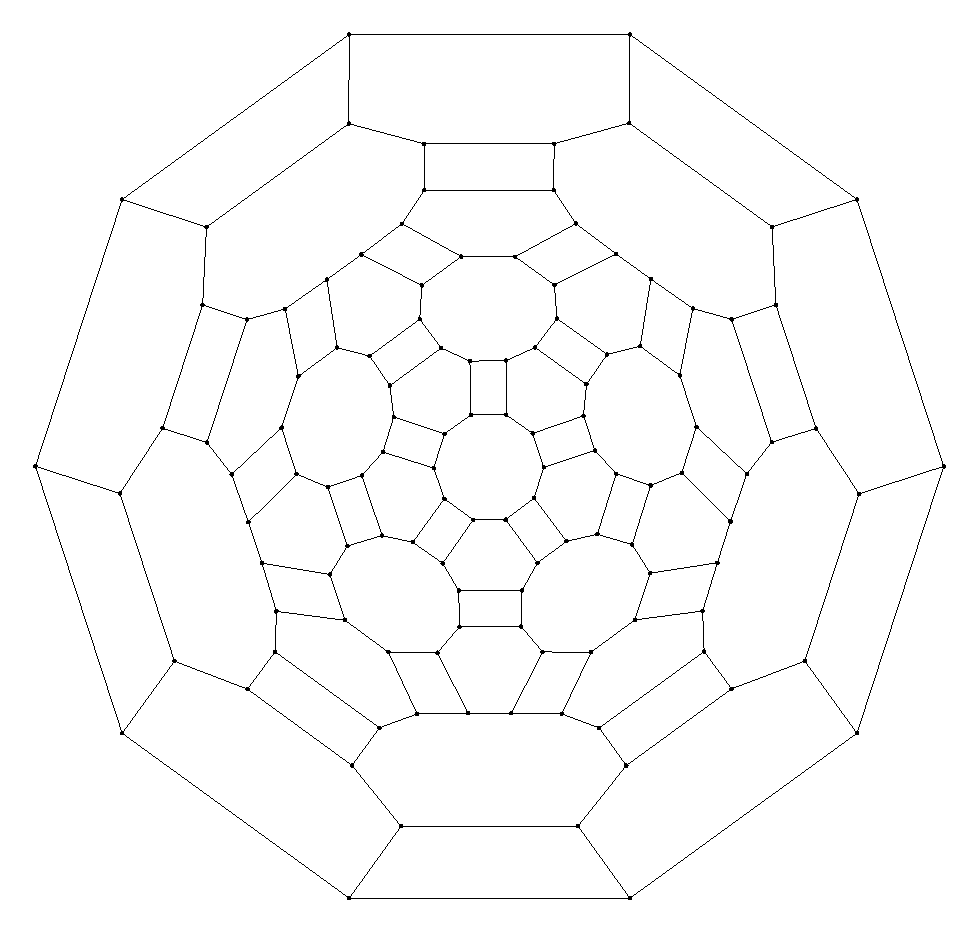
\epsfig{file=GOLDBERGpicture/TruncatedIcosidodecahedron.ps,width=30mm}
\end{center}
\end{minipage}
\begin{minipage}{6cm}
\textcolor{red}{
\begin{tabular}{|l|l|l|}
\hline
$2^{30}, 3^{40}$&
$2^{30}, 5^{24}$&
$3^{20}, 5^{24}$\\
$2^{60}, 3^{20}$&
$2^{60}, 5^{12}$&
$3^{40}, 5^{12}$\\
$2^{90}$&
$3^{60}$&
$5^{36}$\\
$9^{20}$&
$6^{30}$&
$15^{12}$\\
\hline
\end{tabular}
}
\end{minipage}
\end{center}


\end{enumerate}
\end{slide}


%%%%%%%%%%%%%%%%%%%% The (k,l)-product
\begin{slide}{}
\begin{center}
{\Huge 
\begin{tabular*}{7cm}{c}
\\[0.2cm]
\textcolor{blue}{V. }\textcolor{red}{$SL_2(\ZZ)$ action}
\end{tabular*}
}
\end{center}
\end{slide}





%%%%%%%%%%%%%%%%%%%%%   the SL2 
\begin{slide}{$SL_2(\ZZ)$ action?}

${\cal P}(G_0)$ is the set of pairs $(g_1,g_2)$. One has
\begin{equation*}
L\odot_{k,l}R=L \odot_{k-l, l}RL\mbox{~~and~~}L\odot_{k,l} R=RL\odot_{k,l-k} R
\end{equation*}
The matrices $\left(\begin{array}{cc}
1 &0\\
-1&1
\end{array}\right)$ and $\left(\begin{array}{cc}
1 &-1\\
0 &1
\end{array}\right)$ generate $SL_2(\ZZ)$. We want to define $\phi$ such that
\begin{enumerate}
\item[(i)] $\phi$ is a group action of $SL_2(\ZZ)$ on ${\cal P}(G_0)$
\item[(ii)] If $M \in SL_2(\ZZ)$, then the mapping $\phi(M):{\cal P}(G_0)\rightarrow {\cal P}(G_0)$ satisfies
\begin{center}
\begin{tabular}{c}
if $\phi(M)(g_1, g_2)=(h_1, h_2)$\\
then $g_1\odot_{(k,l)M} g_2=h_1 \odot_{k,l} h_2$
\end{tabular}
\end{center}
\end{enumerate}
\textcolor{blue}{This is in fact not possible!}
\end{slide}




\begin{slide}{$SL_2(\ZZ)$ action}

\begin{enumerate}
\item[\ding{108}] $SL_2(\ZZ)$ is generated by matrices
\begin{equation*}
\textcolor{red}{
T=\left(\begin{array}{cc}
0&1\\
-1&0
\end{array}\right)}\mbox{~~and~~}
\textcolor{red}{
U=\left(\begin{array}{cc}
0&1\\
-1&-1
\end{array}\right)}
\end{equation*}
all relation between $T$ and $U$ are generated by the relations 
\begin{equation*}
T^4=I_2,\mbox{~~~}U^3=I_2\mbox{~~and~~}T^2U=UT^2
\end{equation*}
\item[\ding{108}] We write
\begin{equation*}
\begin{array}{rcl}
\textcolor{red}{\phi(T)(g_1,g_2)}&=&\textcolor{red}{(g_2, g_2g_1^{-1}g_2^{-1})}\\
\textcolor{red}{\phi(U)(g_1,g_2)}&=&\textcolor{red}{(g_2, g_2 g_1^{-1}g_2^{-2})}
\end{array}
\end{equation*}


\end{enumerate}
\end{slide}


\begin{slide}{$SL_2(\ZZ)$ action (continued)}
\begin{enumerate}
\item[\ding{224}] By computation
\begin{equation*}
\begin{array}{rcl}
\phi(T)^4(g_1, g_2)&=&Int_{g_1g_2^{-1}g_1^{-1}g_2}(g_1, g_2),\\
\phi(U)^3(g_1, g_2)&=&Int_{g_1g_2^{-1}g_1^{-1}g_2}(g_1, g_2),\\
\phi(T)^2\phi(U)(g_1, g_2)&=&\phi(U)\phi(T)^2(g_1, g_2)\;.
\end{array}
\end{equation*}
\item[\ding{224}] \textcolor{blue}{Group action} of $SL_2(\ZZ)$ on $\QuotS{{\cal P}(G_0)}{D(Mov(G_0))}$.
\item[\ding{224}] If $M$ preserve the element $\overline{(L,R)}$ in $\QuotS{{\cal P}(G_0)}{D(Mov(G_0))}$, then for all pairs $(k,l)$:
\begin{equation*}
GC_{k,l}(G_0)\mbox{~~~~and~~~~}GC_{(k,l)M}(G_0)
\end{equation*}
have the same [ZC] vector. This define a \textcolor{blue}{subgroup of finite index of $SL_2(\ZZ)$}
\end{enumerate}
\end{slide}





%%%%%%%%%    the stabilizer of pairs
%\begin{slide}{$Rot(G_0)$ transitive}
%\begin{enumerate}
%\item[\ding{108}] $Rot(G_0)$ is the subgroup of $Aut(G_0)$ formed by all rotations stabilizing $G_0$
%\item[\ding{108}] its action on ZC-circuit is transitive
%\item[\ding{108}] its action on ${\cal DE}$ is free.
%\item[\ding{108}] action of $Rot(G_0)$ and $Mov(G_0)$ on ${\cal DE}$ commute.
%\item[\ding{108}] If $Rot(G_0)$ is transitive on ${\cal DE}$ then
%\begin{equation*}
%\left\lbrace\begin{array}{rcl}
%\phi_{\overrightarrow{e}}: Mov(G_0)&\rightarrow& Rot(G_0)\\
%u&\mapsto& \phi_{\overrightarrow{e}}(u)
%\end{array}\right.
%\end{equation*}
%with $u^{-1}(\overrightarrow{e})=\phi_{\overrightarrow{e}}(u)(\overrightarrow{e})$, is an injective group morphism. $\phi_{\overrightarrow{e}}(Mov(G_0))$ is normal in $Rot(G_0)$.
%\end{enumerate}
%\end{slide}




%%%%%%%%%%%%%%%%%%%%%%   extremal case
%\begin{slide}{Extremal cases}
%\begin{enumerate}
%\item[\ding{108}] If $Rot(G_0)$ is non-trivial, then there are restriction on $Mov(G_0)$.
%\item[\ding{108}] If $Rot(G_0)$ is transitive on ${\cal DE}$, then $Mov(G_0)$ has at most $3n$ ($3$-valent) or $4n$ ($4$-valent) directed edges
%
%
%\item[\ding{108}] $Mov(G_0)$ is formed of even permutation on $3n$ or $4n$ directed edges.
%\item[\ding{108}] In some cases $Mov(G_0)=Alt(3n)$.
%\begin{center}
%\begin{minipage}[t]{25mm}
%\centering
%\epsfxsize=25mm
%\epsfbox{Explosion1.ps}
%\end{minipage}
%\begin{minipage}[t]{25mm}
%\centering
%\epsfxsize=23mm
%\epsfbox{Explosion2sec.eps}
%\end{minipage}
%\begin{minipage}[t]{25mm}
%\centering
%\epsfxsize=25mm
%\epsfbox{Explosion4.ps}
%\end{minipage}
%\begin{minipage}[t]{25mm}
%\centering
%\epsfxsize=25mm
%\epsfbox{Explosion9.ps}
%\end{minipage}
%\end{center}
%\item[\ding{108}] We have no example of $4$-valent plane graph $G_0$ with $Mov(G_0)=Alt(4n)$.
%\end{enumerate}
%\end{slide}



%%%%%%%%%%%%%%%%%%%%%%   extremal case
%\begin{slide}{$Mov(G_0)$ commutative}
%\begin{enumerate}
%\item[\ding{108}] $Mov(G_0)$ commutative $\Leftrightarrow$  $G_0$ is either a graph $2_n$, a graph $3_n$ or a $4$-hedrite.
%\epsfxsize=10mm
%\item[\ding{108}] Class $2_n$ (Grunbaum-Zaks): Goldberg-Coxeter of the Bundle \epsfbox{Bundle.eps}
%\begin{center}
%\begin{minipage}{5cm}
%\centering
%\epsfig{file=Class3n.eps,width=40mm}
%Class $3_n$ (Grunbaum-Motzkin): 
%\end{minipage}
%\begin{minipage}{5cm}
%\centering
%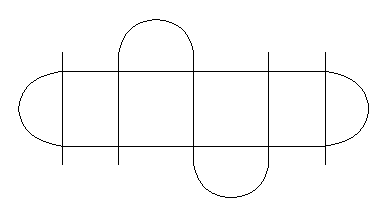
\epsfig{file=Class4hedrite.eps,width=40mm}
%Class $4$-hedrite (Deza-Shtogrin): 
%\end{minipage}
%\end{center}
%
%\end{enumerate}
%\end{slide}




\begin{slide}{}
\begin{center}
{\Huge 
\begin{tabular*}{4cm}{c}
\\[-0.5cm]
\textcolor{red}{Thank}\\
\textcolor{red}{You}
\end{tabular*}
}
\end{center}
\end{slide}



\end{document}
